\documentclass[a4paper, 14pt]{extarticle}

% Поля
%--------------------------------------
\usepackage{geometry}
\geometry{a4paper,tmargin=2cm,bmargin=2cm,lmargin=3cm,rmargin=1cm}
%--------------------------------------


%Russian-specific packages
%--------------------------------------
\usepackage[T2A]{fontenc}
\usepackage[utf8]{inputenc} 
\usepackage[english, main=russian]{babel}
%--------------------------------------

\usepackage{textcomp}

% Красная строка
%--------------------------------------
\usepackage{indentfirst}               
%--------------------------------------             


%Graphics
%--------------------------------------
\usepackage{graphicx}
\graphicspath{ {./images/} }
\usepackage{wrapfig}
%--------------------------------------

% Полуторный интервал
%--------------------------------------
\linespread{1.3}                    
%--------------------------------------

%Выравнивание и переносы
%--------------------------------------
% Избавляемся от переполнений
\sloppy
% Запрещаем разрыв страницы после первой строки абзаца
\clubpenalty=10000
% Запрещаем разрыв страницы после последней строки абзаца
\widowpenalty=10000
%--------------------------------------

%Списки
\usepackage{enumitem}

%Подписи
\usepackage{caption} 

%Гиперссылки
\usepackage{hyperref}

\hypersetup {
	unicode=true
}

%Рисунки
%--------------------------------------
\DeclareCaptionLabelSeparator*{emdash}{~--- }
\captionsetup[figure]{labelsep=emdash,font=onehalfspacing,position=bottom}
%--------------------------------------

\usepackage{tempora}
\usepackage{amsmath}
\usepackage{color}
\usepackage{listings}
\lstset{
  belowcaptionskip=1\baselineskip,
  breaklines=true,
  frame=L,
  xleftmargin=\parindent,
  language=Python,
  showstringspaces=false,
  basicstyle=\footnotesize\ttfamily,
  keywordstyle=\bfseries\color{blue},
  commentstyle=\itshape\color{purple},
  identifierstyle=\color{black},
  stringstyle=\color{red},
}

%--------------------------------------
%			НАЧАЛО ДОКУМЕНТА
%--------------------------------------

\begin{document}

%--------------------------------------
%			ТИТУЛЬНЫЙ ЛИСТ
%--------------------------------------
\begin{titlepage}
\thispagestyle{empty}
\newpage


%Шапка титульного листа
%--------------------------------------
\vspace*{-60pt}
\hspace{-65pt}
\begin{minipage}{0.3\textwidth}
\hspace*{-20pt}\centering

\includegraphics[width=\textwidth]{emblem}
\end{minipage}
\begin{minipage}{0.67\textwidth}\small \textbf{
\vspace*{-0.7ex}
\hspace*{-6pt}\centerline{Министерство науки и высшего образования Российской Федерации}
\vspace*{-0.7ex}
\centerline{Федеральное государственное бюджетное образовательное учреждение }
\vspace*{-0.7ex}
\centerline{высшего образования}
\vspace*{-0.7ex}
\centerline{<<Московский государственный технический университет}
\vspace*{-0.7ex}
\centerline{имени Н.Э. Баумана}
\vspace*{-0.7ex}
\centerline{(национальный исследовательский университет)>>}
\vspace*{-0.7ex}
\centerline{(МГТУ им. Н.Э. Баумана)}}
\end{minipage}
%--------------------------------------

%Полосы
%--------------------------------------
\vspace{-25pt}
\hspace{-35pt}\rule{\textwidth}{2.3pt}

\vspace*{-20.3pt}
\hspace{-35pt}\rule{\textwidth}{0.4pt}
%--------------------------------------

\vspace{1.5ex}
\hspace{-35pt} \noindent \small ФАКУЛЬТЕТ\hspace{80pt} <<Информатика и системы управления>>

\vspace*{-16pt}
\hspace{47pt}\rule{0.83\textwidth}{0.4pt}

\vspace{0.5ex}
\hspace{-35pt} \noindent \small КАФЕДРА\hspace{50pt} <<Прикладная Математика и информатика>>

\vspace*{-16pt}
\hspace{30pt}\rule{0.866\textwidth}{0.4pt}
  
\vspace{11em}

\begin{center}
\Large {\bf "Летучка" 2} \\ 
\large {\bf по курсу <<Языки и методы программирования>>} \\ 
\large <<Модель вселенной>>
\end{center}\normalsize

\vspace{8em}


\begin{flushright}
  {Студент группы ИУ9-21Б Хромов М.А.\hspace*{15pt} \\
  \vspace{2ex}
  Преподаватель Посевин Д. П.\hspace*{15pt}}
\end{flushright}

\bigskip

\vfill
 

\begin{center}
\textsl{Москва 2025}
\end{center}
\end{titlepage}
%--------------------------------------
%		КОНЕЦ ТИТУЛЬНОГО ЛИСТА
%--------------------------------------

\renewcommand{\ttdefault}{pcr}

\setlength{\tabcolsep}{3pt}
\newpage


 

\section{Задание}\label{Sect::task}
\par
Реализовать модель вселенной. Каждый элемент вселенной должен быть объектом некоего публичного класса, который инициализируется вспомогательным публичным классом порождающим эту вселенную. При инициализации экземпляров класса частиц моделируемой вселенной необходимо подсчитывать количество частиц вселенной используя статичное экземплярное поле защищенное от изменения из объектов внешних классов путем реализации статичного метода. Сформировать исходные данные и определить необходимые экземплярные поля для хранения состояния объектов частиц вселенной в соответствии с условием задачи и реализовать расчет.  
	Программа должна обладать консольным пользовательским интерфейсом ввода данных, например, количества частиц вселенной, масс частиц и т.д.


\section{Индивидуальный вариант}\label{Sect::task}
\par
Вычислить силу притяжения действующую на произвольную частицу массой M находящейся в заданной координате пространства со стороны всех частиц вселенной.
\section {Практическая реализация}
Исходный код программы представлен в листингах 1-4
\begin{figure}[!htb]
\begin{lstlisting}[language={},caption={класс},label={lst:code1}]
public class GravityCalculator {
    public static double[] calculateForce(Universe universe, double m, double x, double y, double z) {
        double fx = 0, fy = 0, fz = 0;

        for (Particle p : universe.getParticles()) {
            double dx = p.getX() - x;
            double dy = p.getY() - y;
            double dz = p.getZ() - z;
            double distanceSquared = dx * dx + dy * dy + dz * dz;

            if (distanceSquared < 1e-10) continue;

            double distance = Math.sqrt(distanceSquared);
            double force = (Particle.G * m * p.getMass()) / distanceSquared;

            fx += force * (dx / distance);
            fy += force * (dy / distance);
            fz += force * (dz / distance);
        }

        return new double[]{fx, fy, fz};
    }
}

\end{lstlisting}
\end{figure}
\begin{figure}[!htb]
\begin{lstlisting}[language={},caption={класс},label={lst:code2}]
public class Particle {
    private static int particleCount = 0;
    public static final double G = 6.67430e-11;
    private double mass;
    private double x, y, z;

    public Particle(double mass, double x, double y, double z) {
        this.mass = mass;
        this.x = x;
        this.y = y;
        this.z = z;
        particleCount++;
    }

    public static int getParticleCount() {
        return particleCount;
    }

    public double getMass() { return mass; }
    public double getX() { return x; }
    public double getY() { return y; }
    public double getZ() { return z; }
}

\end{lstlisting}
\end{figure}

\begin{figure}[!htb]
\begin{lstlisting}[language={},caption={класс},label={lst:code3}]
import java.util.ArrayList;
import java.util.List;

public class Universe {
    private List<Particle> particles;

    public Universe() {
        particles = new ArrayList<>();
    }

    public void addParticle(double mass, double x, double y, double z) {
        particles.add(new Particle(mass, x, y, z));
    }

    public List<Particle> getParticles() {
        return particles;
    }
}

\end{lstlisting}
\end{figure}

\begin{figure}[!htb]
\begin{lstlisting}[language={},caption={класс},label={lst:code4}]
import java.util.Scanner;

public class UniverseSimulation {
    public static void main(String[] args) {
        Scanner scanner = new Scanner(System.in);
        Universe universe = new Universe();

        System.out.print("количество частиц во вселенной: ");
        int n = scanner.nextInt();

        for (int i = 0; i < n; i++) {
            System.out.println("параметры частицы " + (i + 1) + " (масса, x, y, z):");
            double mass = scanner.nextDouble();
            double x = scanner.nextDouble();
            double y = scanner.nextDouble();
            double z = scanner.nextDouble();
            universe.addParticle(mass, x, y, z);
        }

        System.out.println("частиц во вселенной: " + Particle.getParticleCount());

        System.out.println("координаты частицы (тестовой (не нуждается во вселенной) для расчета силы (масса, x, y, z):");
        double m = scanner.nextDouble();
        double x = scanner.nextDouble();
        double y = scanner.nextDouble();
        double z = scanner.nextDouble();

        double[] force = GravityCalculator.calculateForce(universe, m, x, y, z);

        System.out.printf("Сила притяжения: Fx = %.5e, Fy = %.5e, Fz = %.5e\n", force[0], force[1], force[2]);

        scanner.close();
    }
}

\end{lstlisting}
\end{figure}

\clearpage


\section{Реализация}

\begin{center}
    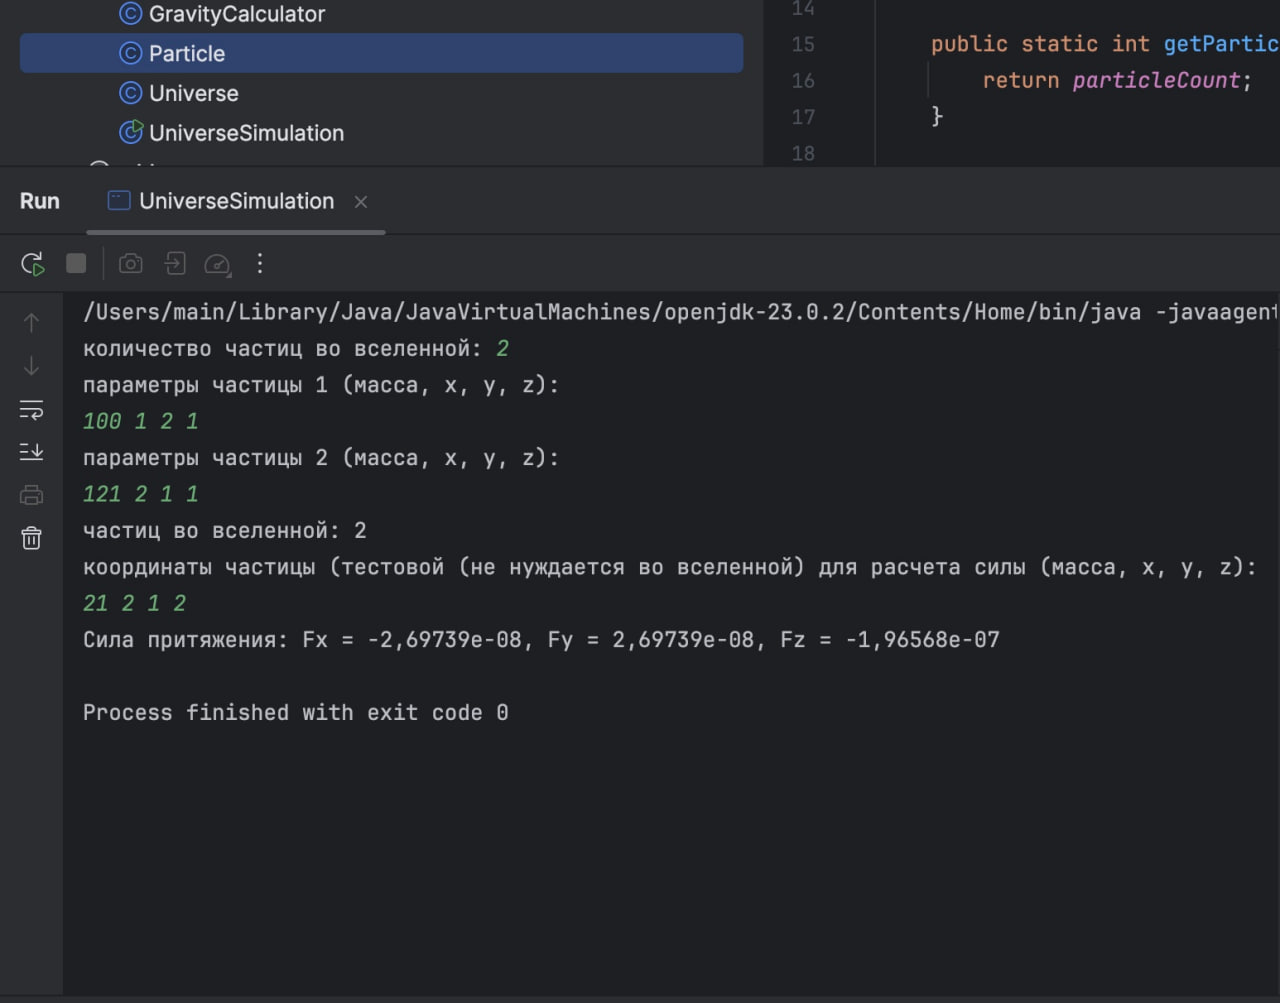
\includegraphics[width=0.8\textwidth]{фото17.jpeg}
    \captionof{figure}{вывод}
\end{center}
\newpage
\section{Вывод}
В ходе работы была реализована модель вселенной на языке Java, включающая классы Particle, Universe и GravityCalculator. Основные задачи:

Инкапсуляция: Состояние частиц (масса, координаты) защищено приватными полями, доступ через геттеры.

Статический счетчик: Количество частиц отслеживается через статическое поле particleCount.

Расчет силы притяжения: Реализован метод calculateForce(), вычисляющий силу по закону всемирного тяготения.

Консольный интерфейс: Пользователь может задавать параметры частиц и тестовой точки для расчета.

\end{document}